\subsection{Singleton}
\begin{flushleft}
    Ngoài 3 Design Patterns chính, nhóm còn sử dụng thêm một Design Pattern khác, đó là \textit{Singleton}.~\textbf{Singleton} là một Design Pattern cung cấp một cách để giới hạn việc tạo ra một đối tượng của một lớp đến một đối tượng duy nhất. Điều này đảm bảo rằng một lớp chỉ có một thể hiện và cung cấp một cách để truy cập nó.

    \begin{figure}[H]
        \centering
        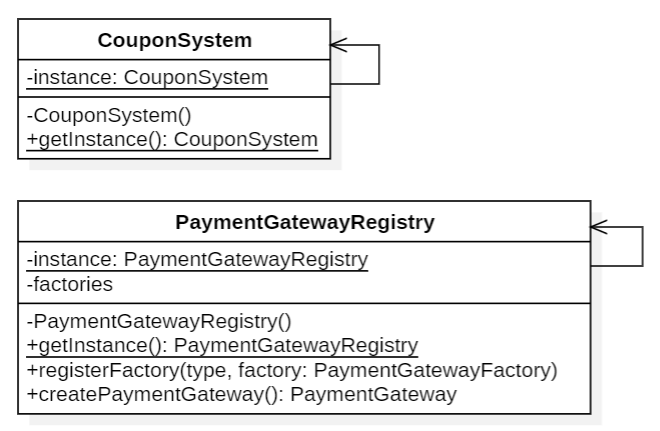
\includegraphics[width=0.9\textwidth]{../assets/screenshots/uml/singleton.png}
        \caption{Factory Method UML Class Diagram}
    \end{figure}

    \begin{itemize}
        \item \textbf{CouponSystem}:
              \begin{itemize}
                  \item \textbf{Vai trò:} Là điểm vào duy nhất để truy cập các chức năng liên quan đến mã giảm giá, như áp dụng mã giảm giá cho đơn hàng, chứa các logic kiểm tra tính hợp lệ của mã giảm giá, quản lý thời hạn sử dụng, v.v.
              \end{itemize}
        \item \textbf{PaymentGatewayRegistry}:
              \begin{itemize}
                  \item \textbf{Vai trò:} Là một registry để quản lý các phương thức thanh toán khác nhau, cho phép hệ thống thêm các phương thức thanh toán mới một cách linh hoạt bằng cách đăng ký các factory tương ứng.
              \end{itemize}
    \end{itemize}
\end{flushleft}
